%%
%% This is file `squelette-rr.tex',
%% generated with the docstrip utility.
%%
%% The original source files were:
%%
%% RR.dtx  (with options: `sample')
%% ********************************************************************
%% Copyright (C) 1997-1999 2004 2006-2010 INRIA/APICS by Jose' Grimm
%% This file may be distributed and/or modified under the
%% conditions of the LaTeX Project Public License, either version 1.3
%% of this license or (at your option) any later version.
%% The latest version of this license is in
%%    http://www.latex-project.org/lppl.txt
%% and version 1.3 or later is part of all distributions of LaTeX
%% version 2003/12/01 or later.
%% An archive of the software can be found at
%%    ftp://ftp-sop.inria.fr/apics/rr-inria

\documentclass[a4paper]{article}
\usepackage[latin1]{inputenc} % ou \usepackage[utf8]{inputenc}
\usepackage[T1]{fontenc} % ou \usepackage[OT1]{fontenc}
\usepackage{RR,RRthemes}
\usepackage{hyperref}
\usepackage{listings}
\usepackage{verbatim}
\usepackage{graphicx}
\usepackage{color}
%%\usepackage[frenchb]{babel} % optionnel
%%
%% date de publication du rapport
\RRdate{Juin 2011}
%%
%% Cas d'une version deux
%% \RRversion{2}
%% date de publication de la version 2
%% \RRdater{Novembre  2006}
\usepackage{listings}

\usepackage{amssymb}
\usepackage{xspace} 
\usepackage{array} 
\usepackage{multirow}
\newcommand\hyph{\nobreak\hskip0pt-\nobreak\hskip0pt\relax}
\newlength\savedwidth
\newcommand\whline{\noalign{\global\savedwidth
  \arrayrulewidth\global\arrayrulewidth 1.5pt}
  \hline \noalign{\global\arrayrulewidth
  \savedwidth}
}
\newcolumntype{I}{!{\vrule width 1.5pt}}
\renewcommand{\arraystretch}{1.5}

\newcommand{\kaapi}{\textsc{X-Kaapi}\xspace}



%%
\RRauthor{% les auteurs
 % Premier auteur, avec une note
Fabien Le Mentec%
  % note partag\'ee (optionnelle)
%  \thanks[sfn]{Shared foot note}%
 % \and entre chaque auteur s'il y en a plusieurs
  \and
Thierry Gautier%\thanks{Footnote for second author}%
 % r\'ef\'erence \`a la note partag\'ee
%\thanksref{sfn}
  \and
Vincent Danjean%\thanks{Footnote for second author}%
 % r\'ef\'erence \`a la note partag\'ee
%\thanksref{sfn}
}
%%
%% Ceci apparait sur chaque page paire.
\authorhead{Le Mentec \& Gautier & Danjean}
%%
\RRtitle{The \kaapi's programming model and user's manual}
%% English title
\RRetitle{The \kaapi's programming model \\and \\User's manual}
%%
\titlehead{The \kaapi's programming model}
%%
%\RRnote{This is a note}
%\RRnote{This is a second note}
%%
\RRresume{
}
\RRabstract{During the past years, dynamically scheduled data flow graphs for tiled algorithms in linear algebra have appeared as a promising way to reach the portability of performance onto several multicore architectures.
The idea was to describe those algorithms as an abstract data flow graph representation that only encodes tasks and their dependencies independently of the scheduling algorithm, which folds up tasks onto the cores of the target architecture. 
Reported experimental timings show good performances for linear algebra algorithms where tasks are generated only from nested loops. Nevertheless, all recently proposed frameworks do not consider programs where tasks with data flow dependencies are generated recursively. 

In this report, we present \kaapi's programming model. A parallel \kaapi program is a C or C++ sequential program with code annotation using \texttt{\#pragma} compiler directives. A specific source to source compiler translates \kaapi directives to runtime calls.
}

%%
\RRmotcle{}
\RRkeyword{parallel computing, data flow graph, locality guided work stealing, \kaapi}
%%
%% \RRprojet{Apics}  % cas d'un seul projet
\RRprojets{MOAIS}
\RRdomaine{3} % cas du domaine numero 1
\RRthemeProj{moais} % theme du projet Apics
%\RRdomaineProjBis{apics} % domaine du projet Apics
%% \RRdomaineProjBis{pop art} % domaine du projet PopArt
%%
%% \URLorraine % pour ceux qui sont \`a l'est
%% \URRennes  % pour ceux qui sont \`a l'ouest
%% \URRhoneAlpes % pour ceux qui sont dans les montagnes
%% \URRocq % pour ceux qui sont au centre de la France
%% \URFuturs % pour ceux qui sont dans le virtuel
%% \URSophia % pour ceux qui sont au Sud.
%%
%% \RCBordeaux % centre de recherche Bordeaux - Sud Ouest
%% \RCLille % centre de recherche Lille Nord Europe
%% \RCParis % Paris Rocquencourt
%% \RCSaclay % Saclay \^Ile de France
\RCGrenoble % Grenoble - Rh\^one-Alpes
%% \RCNancy % Nancy - Grand Est
%% \RCRennes % Rennes - Bretagne Atlantique
%\RCSophia % Sophia Antipolis M\'editerran\'ee

%%
\begin{document}
%%
%\makeRR   % cas d'un rapport de recherche
\makeRT % cas d'un rapport technique.
%% a partir d'ici, chacun fait comme il le souhaite


\tableofcontents


\newpage
\section{Context}

Several research projects~\cite{Gunnels:2001:FFL,plasma-analysis,PerezBL08} have investigated the use of data flow graphs as an intermediate representation of the computation of LAPACK's algebra algorithms~\cite{plasma-lapack}: the main reason was that the portability of performance in LAPACK is of the responsibility of a set of basic linear algebra subprograms (BLAS), which exhibit only a low level parallelism that is not enough on multicores.

Without taking care of considerations about tile algorithms to reach performances, three majors points have been identified as important to perform efficient tile algorithms~\cite{Gunnels:2001:FFL,plasma-analysis,plasma-lapack}: 1/ fine granularity to reach high level of parallelism; 2/ asynchronous execution to prevent barrier of synchronization; and 3/ a dynamic data driven scheduler to ensure execution of task as soon as all their input data are produced.

Point 1/ was already mentioned since the first papers about Cilk~\cite{Cilk5:1998} and formalized in the Cilk performance model~\cite{CilkSched98} where the parallel time is lower bounded by the critical path: a program that cannot exploit fine grain parallelism is difficult to schedule with guaranted linear speed up, even for a reasonable number of processors.
Points 2/  and 3/ are at the basis of the execution of data flow machines~\cite{dataflow} or languages~\cite{Jade:1998, Athapascan98} that try to schedule instructions as soon as input operands are produced.


Nevertheless, most of the recently proposed frameworks that share the data flow graph as a central representation to dynamically schedule tasks according to their dependencies, are not able to run programs with recursive tasks creations.  

This report presents \kaapi, a runtime library and a source to source compiler to program NUMA multicore machines.
\kaapi is based on a macro data flow graph: the sequential code is annotated to identify functions to be transformed into tasks. Each function that is candidate to become a task must be annotated in order to specify the access mode (read, write, reduction, exclusive) made through its parameter to the memory. The compiler will insert task creations and the runtime will detect the dependencies and schedule the tasks onto the cores.

The \kaapi programming model comes from Athapascan~\cite{Athapascan98} which, itself, was inspired by Jade~\cite{Jade:1998} and Cilk~\cite{Cilk5:1998}. Because the \kaapi programming model and  StarSs~\cite{Badia:2009} are very closed, we also accept the execution of StarSs program. Descriptions of \kaapi may be found in following publications~\cite{Kaapi_2007,Traore_2008-deque_free, CCK_MCO08,KAAPI_TIC_2009}.

This technical report is organized as follows. FIXME Section~\ref{sec:helloworld} presents 
though simple examples how to program with \kaapi in C or C++.

%%%
%%%
\newpage
\section{Software installation}\label{sec:userinstall}

\kaapi is both a programming model and a runtime for high performance parallelism targeting multicore and distributed architectures. 
It relies on the work stealing paradigm.
\kaapi was developed in the MOAIS INRIA project by Thierry Gautier, Fabien Le Mentec, Vincent Danjean and Christophe Laferri�re in the early stage of the library.

In this report, only the programming model based on code annotations with \texttt{pragma} compiler directives is presented.
The runtime library comes also with a full set of complementary programming interfaces: C, C++ and STL-like interfaces. The C++ and STL interfaces, at a higher level than the C interface, may be directly used for developing parallel programs or libraries.

\subsubsection*{Supported Platforms}
\kaapi targets essentially SMP and NUMA platforms. The runtime should run
on any system providing:
\begin{itemize}
\item a GNU toolchain (4.3),
\item the pthread library,
\item Unix based environment.
\end{itemize}
It has been extensively tested on the following operating systems:
GNU-Linux/x86\_64 and MacOSX/Intel processor.
There is no version for Windows yet.

\subsubsection*{\kaapi Contacts}
If you wish to contact the XKaapi team, please visite the web site at:
\begin{center}
\url{http://kaapi.gforge.inria.fr}
\end{center}


\subsection{Installation}

To install \kaapi programming model and compiler you need to:
\begin{itemize}
\item install the \kaapi libraries and runtime
\item install the compiler
\end{itemize}
The \kaapi libraries and runtime are available at \url{http://kaapi.gforge.inria.fr} (tarball) or as a Debian package. \kaapi libraries and runtime are distributed under a CeCILL-C license\footnote{\url{http://www.cecill.info/index.en.html} for english version}:
\begin{center}
\begin{minipage}{0.9\linewidth}
\it
CeCILL-C is well suited to libraries and more generally software components. Anyone distributing an application which includes components under the CeCILL-C license must mention this fact and make any changes to the source code of those components available to the community under CECILL-C while being free to choose the licence of its application.\end{minipage}
\end{center}

Moreover, the \kaapi compiler is based on the ROSE\footnote{\url{http://www.rosecompiler.org}} framework to develop source-to-source translators. In this framework, the C and C++ frontends are based on the EDG frontend. 
ROSE is available under a BSD license, but the binary code for EDG must be downloaded separately. 

\subsubsection{ROSE and EDG frontend installation}
The ROSE framework (\url{http://www.rosecompiler.org/}) must be installed. Please have a look at the installation guide on the ROSE web site.

In order to install ROSE, you need to have (valid for ROSE 0.9.5a):
\begin{itemize}
\item \texttt{wget}: to download the binary version of the EDG frontend
\item \texttt{gcc, g++}: at least version 4.0.0
\item \texttt{boost}: version 1.36.0 to 1.45.0
\item and a lot of different utilities (GNU autotools, ...)
\end{itemize}
Detailed procedures to install ROSE and EDG frontend are described in ROSE documents.

Once ROSE is installed, you will be able to generate \verb+kacc+, the \kaapi compiler.

\subsubsection{\kaapi library installation}
There are 2 ways to install \kaapi:
\begin{itemize}
\item using the Debian packages,
\item installing from source.
\end{itemize}

%% sub
\subsubsection*{Using the Debian packages}
Below is a list of the Debian packages provided for using and programming with \kaapi. \\
\textit{
TODO: d�crire ici le package n�cessaire pour le compilateur. A priori uniquement la lib C + �ventuellement une lib C++ pour des classes tableaux et/ou autre data structure qui serait d�j� 'pr�-d�finie' pour �tre passer correctement en param�tre de t�che. Je pense ici � la lib des array/range2D qui permet facilement de faire de la d�coupe r�cursive de donn�es.
}
%% sub
\subsubsection*{Installing from sources}

There are 2 ways to retrieve the sources:
\begin{itemize}
\item download a release snapshot at the following url:\newline
\url{https://gforge.inria.fr/frs/?group_id=94}.
\item clone the git repository of the project:\newline
\verb+> git clone git://git.ligforge.imag.fr/git/kaapi/xkaapi.git xkaapi+
\end{itemize}
\textit{
TODO: GIT anonymous ou non ? A pr�ciser comment rejoindre le projet si volont�.
}


\paragraph{Configuration.}
The build system uses GNU Autotools.
In case you cloned the project repository, you first have to bootstrap the
configuration process by running the following script:
\begin{verbatim}
$> ./bootstrap
\end{verbatim}
The \textit{configure} file should be present. It is used to create the
\textit{Makefile} accordingly to your system configuration. Command line
options can be used to modify the default behavior. You can have a complete
list of the available options by running:
\begin{verbatim}
$> ./configure --help
\end{verbatim}


Below is a list of the most important ones:
\begin{itemize} %% option list
\item \verb+--enable-mode=debug+ or \verb+release+\newline
Choose the compilation mode of the library. Defaults to release.
\item \verb+--with-perfcounter+\newline
Enable performance counters support.
\item \verb+--with-papi+\newline
Enable the PAPI library for low level performance counting.
More information on PAPI can be found at http://icl.cs.utk.edu/papi/.
\item \verb+--enable-kacc+\newline \textbf{required} to compile the \verb+kacc+ compiler.
Depending on your installation of ROSE and the Boost library, you may specify their installation paths using:\\
\hspace*{4ex}\verb+--with-rose=<rose installation>+ \\
or\\
\hspace*{4ex} \verb+--with-boost=<boost installation>+
\item \verb+--prefix=+\newline
Overload the default installation path.
\end{itemize} %% option list
Example:

\begin{verbatim}
./configure --enable-mode=release --prefix=$HOME/install
\end{verbatim}
If there are errors during the configuration process, you have to solve
them before going further. If dependencies are missing on your
system, logs will give you the names of the software to install.

\paragraph{Compilation and installation.}
On success, the configuration process generates a Makefile. The 2 following
commands build and install the \kaapi runtime:
\begin{verbatim}
$> make
$> make install
\end{verbatim}

\paragraph{Checking the installation.}
The following checks that the runtime is correctly installed on your system:
\begin{verbatim}
$> make check
\end{verbatim}

\paragraph{Compilation of the examples.}
The following compiles the sample applications:
\begin{verbatim}
$> cd examples; make examples
\end{verbatim}

\subsubsection*{Installation directory}

The configure, make, make install, commands create in the prefix directory the following 
directory structure:
\begin{verbatim}
<prefix>/include
<prefix>/lib
<prefix>/bin
<prefix>/share
\end{verbatim}

The KaCC compiler is located in \texttt{<prefix>/bin}, it should be in your \texttt{\$PATH} variable to avoid full path naming.
All programs compiled with KaCC are linked against libraries located in  \texttt{<prefix>/lib}. 
Executables linked with KaCC do not require to add this directory in your \verb+LD_LIBRARY_PATH+ (under linux) or \verb+DYLD_LIBRARY_PATH+ (under Mac OS X).

The \texttt{<prefix>/share} directory contains some documentation and examples.

\newpage\section{Getting started}\label{sec:helloworld}

The source distribution of \kaapi contains the repository \verb+examples+. Each subdirectory is dedicated to a problem (fibonacci, matrix product, ...). 
The examples that come with the compiler are located in \verb+examples/compiler+.
A presentation of examples using directly the \kaapi library (with C, C++ or STL) interface is out of the scope of this report.

In the remaining, we only present the \kaapi programming model and we show examples using the \verb+kacc+ compiler only. The process of describing a parallel program with \kaapi is:
\begin{itemize}
\item \kaapi is task based parallel programming model: the user should indicate where task are.
\item A task is a function call without side effect: the user must annotate the code to specify what function is a task. 
\item The compiler will insert task creation code for each appropriate function call.
\item Dependencies between tasks are automatically computed by the runtime through data flow analysis between function calls: when a function is annotated as a task, the user must specify the access mode to the memory for each formal parameter. 
\end{itemize}
All the annotations are specified by pragma directives with the form:
\begin{center}
\texttt{\#pragma kaapi <clause specification>}
\end{center}

\subsection{Hello World}
The example of figure~\ref{ex:helloworld} presents the creation of one task that display "Hello world". The
\kaapi \verb+kacc+ compiler is based on pragma annotations to describe the parallelism, as for OpenMP.

First it is necessary to start a parallel region where tasks may be executed concurrently.
Outside a parallel region tasks are executed only by the current thread. 
This is indicated by \texttt{\#pragma kaapi parallel} at line 11. 
The parallel region begins at the next basic block (between \verb+{+ and \verb+}+) and it ends at the end of the basic block. 
Without brackets it only concerns the following statement.
%It could also be defined before any instruction and it will end after the instruction.

The \texttt{\#pragma kaapi parallel} defines a region where concurrent executions may occur. The number of threads used to execute tasks inside a parallel region may vary during the execution. 
All tasks created inside a parallel region are guaranteed to be completed at the end of the parallel region.

\begin{figure}[ht]
\begin{center}
\begin{minipage}{0.99\linewidth}
\begin{footnotesize}
\lstset{numbers=left, numberstyle=\tiny, stepnumber=1, numbersep=5pt}
\lstset{commentstyle=\color{blue}}
\lstset{language=C}
\begin{lstlisting}[frame=tb]
#include <stdio.h>

#pragma kaapi task value(msg)
void say_hello(const char* msg)
{
  printf("%s\n", msg);
}

int main(int argc, char** argv)
{
#pragma kaapi parallel
    say_hello("Hello World!");
  return 0;
}
\end{lstlisting}
\end{footnotesize}
\end{minipage}
\end{center}
\caption{hello\_world1.c example}\label{ex:helloworld}
\end{figure}
The task in the figure takes one parameter (a C string) and displays it to the screen. The parameter is passed by value: this is specified by the clause \texttt{value(msg)} that tells the compiler the effective parameter is considered as being passed by value. We will see in the following sections what it means.


\subsubsection{Compilation}
To compile the previous example, simply type:
\begin{verbatim}
> kacc -o hello_world hello_world.c
\end{verbatim}
Then, run it with:
\begin{verbatim}
> ./hello_world
Hello World!
\end{verbatim}

This simple example only creates one task without real concurrency\footnote{In fact, there is concurrency between the task execution and the code executed between the end of the function call at line 12 and before the instruction at line 13: it is possible that the task is theft and executed by another thread than the main thread. Nevertheless, at the end of the parallel region, the task is completed.}.

\subsubsection{Two Hello World}

The next example in figure~\ref{ex:helloworld2} creates 2 independent tasks that display two messages.
\begin{figure}[h]
\begin{center}
\begin{minipage}{0.99\linewidth}
\begin{footnotesize}
\lstset{numbers=left, numberstyle=\tiny, stepnumber=1, numbersep=5pt}
\lstset{commentstyle=\color{blue}}
\lstset{language=C}
\begin{lstlisting}[frame=tb]
#include <stdio.h>

#pragma kaapi task value(msg)
void say_hello(const char* msg)
{
  printf("%s\n", msg);
}

int main(int argc, char** argv)
{
#pragma kaapi parallel 
  {
    say_hello("First call: Hello World!");
    say_hello("Second call: Hello World!");
  }
  return 0;
}
\end{lstlisting}
\end{footnotesize}
\end{minipage}
\end{center}
\caption{hello\_world2.c example}\label{ex:helloworld2}
\end{figure}

After compilation and execution we hope to have such output:
\begin{verbatim}
> ./hello_world2
First call: Hello World!
Second call: Hello World!
\end{verbatim}

Moreover, some execution may produce the following output:
\begin{verbatim}
> ./hello_world2
Second call: Hello World!
First call: Hello World!
\end{verbatim}

In \kaapi the task creation is a non-blocking operation: the thread that creates tasks never waits for the completion of the tasks if it is not specified by the user.  All tasks created into a parallel region are guaranteed to be completed at the end of the parallel region: the end of a parallel region has an implicit synchronization point that forces execution of tasks.  But inside a parallel region, tasks may be executed in \textbf{any order} that respects the data flow dependencies between tasks. In the example, tasks have been declared as taking their parameter by value so they are independent.

The three ways \kaapi offers to enforce an execution order are:
\begin{itemize}
\item Tasks have declared special access modes to their parameters (read, write, exclusive), which introduce read-after-write data flow dependencies between tasks: they are the only dependencies that \kaapi respect at runtime. This is the subject of the next section.

\item If tasks are independent, then the user may introduce a synchronization point using the \texttt{\#pragma kaapi sync} directive to force all tasks created in the same function body before the synchronization point to be completed at the end of the synchronization point. In the previous example, this directive must be placed between line 13 and line 14:
\begin{footnotesize}
\lstset{numbers=left, numberstyle=\tiny, stepnumber=1, numbersep=5pt}
\lstset{commentstyle=\color{blue}}
\lstset{language=C}
\begin{lstlisting}[frame=tb, firstnumber=11]
#pragma kaapi parallel
  {
    say_hello("First call: Hello World!");
#pragma kaapi sync
    say_hello("Second call: Hello World!");
  }
\end{lstlisting}
\end{footnotesize}

\item The user may also define a sequence of parallel regions in order to take benefit of the implicit synchronization at the end of each parallel region.
The code of figure~\ref{ex:helloworld2} then becomes:
\begin{footnotesize}
\lstset{numbers=left, numberstyle=\tiny, stepnumber=1, numbersep=5pt}
\lstset{commentstyle=\color{blue}}
\lstset{language=C}
\begin{lstlisting}[frame=tb,, firstnumber=11]
#pragma kaapi parallel
    say_hello("First call: Hello World!");
#pragma kaapi parallel
    say_hello("Second call: Hello World!");
\end{lstlisting}
\end{footnotesize}

\end{itemize}


\subsection{A simple writer-reader scheme}

The example of figure~\ref{ex:simpleWR} creates two tasks in a parallel region defined at line 18. The tasks are created at line 20 and 22.
\begin{figure}[ht]
%\hrule\vspace*{2ex}
\begin{center}
\begin{minipage}{0.99\linewidth}
\begin{footnotesize}
\lstset{numbers=left, numberstyle=\tiny, stepnumber=1, numbersep=5pt}
\lstset{commentstyle=\color{blue}}
\lstset{language=C}
\begin{lstlisting}[frame=tb]
#include <stdio.h>

#pragma kaapi task write(buffer[size]) value(size) read(msg)
void write_msg(int size, char* buffer, const char* msg)
{
  snprintf(buffer, size, "%s", msg);
}

#pragma kaapi task read(msg)
void print_msg(const char* msg)
{
  printf("%s\n", msg);
}

int main(int argc, char** argv)
{
  char buffer[32];
  #pragma kaapi parallel 
  {
    write_msg(32,buffer, 
      "This is a long message for the buffer.");
    print_msg(buffer);
  }

  return 0;
}
\end{lstlisting}
\end{footnotesize}
\end{minipage}
\end{center}
\caption{simple\_prodcons.c example}\label{ex:simpleWR}
\end{figure}


The first task takes 3 parameters: the first one is the size of the buffer which is given as the second parameter. A third parameter points to the message to copy into the buffer. The respective access modes for these parameters, defined at line 3, are:
\begin{itemize}
\item \textbf{by value access mode}, for the parameter \texttt{size} defined by \texttt{'value(size)'}. 
This access mode is like the pass-by-value rule of a C/C++ function call: The callee copies the effective parameter\footnote{The expression passed in the function call.} to the formal parameter\footnote{The name of the variable in the function definition}. The callee receives a copy of the value that can be modified. Modifications are not viewed by the caller.
\item \textbf{write access mode} of \texttt{buffer} defined by \texttt{'write(buffer[size])'}. 
In this example, the function writes characters into a buffer. 
The clause specifies the size of the buffer (\texttt{buffer[size]}) written by the task.
Modifications of the buffer during task execution are reported to the callee. 
With this access mode, the input value of the parameter \texttt{buffer} is unspecified.

\item \textbf{read access mode} for the variable \texttt{msg} defined by \texttt{'read(msg)'}.
This parameter is the C string read by the task and copied into the parameter \texttt{buffer}.
The size of the string follows the C convention  of null terminated string.
\end{itemize}

The second task declares (line 9) that it reads its single parameter.

The same effective parameter \texttt{buffer}, declared at line 17,�is passed between the two tasks at line 20 and 21. Because of the previous declaration of \texttt{write} access in the first task and \texttt{read} access in the second task, it induces a \textbf{true} data flow dependency between the tasks.

In \kaapi, any parameter that has to be shared between tasks must be a pointer to a data structure. In the previous example, it is a C-string, \textit{i.e.} a pointer to a null terminated array of characters.


\subsection{Recursive computation: Fibonacci}
The figure~\ref{ex:fibonacci} presents a recursive computation of the $n$-th Fibonacci number\footnote{For simplification, $n$ was fixed to 30 in the code.} using the classical non optimal algorithm.

\begin{figure}[ht]
\begin{center}
\begin{minipage}{0.99\linewidth}
\begin{footnotesize}
\lstset{numbers=left, numberstyle=\tiny, stepnumber=1, numbersep=5pt}
\lstset{commentstyle=\color{blue}}
\lstset{language=C}
\begin{lstlisting}[frame=tb]
#include <stdio.h>

#pragma kaapi task write(result) value(n)
void fibonacci(long* result, const long n)
{
  if (n<2)
    *result = n;
  else 
  {
    long r1,r2;
    fibonacci( &r1, n-1 );
    fibonacci( &r2, n-2 );
#pragma kaapi sync
    *result = r1 + r2;
  }
}

#pragma kaapi task read(result) 
void print_result( const long* result )
{
  printf("Fibonacci(30)=%li\n", *result);
}

int main()
{
  long result;
#pragma kaapi parallel
  {
    fibonacci(&result, 30);
    print_result(&result);
  }
  return 0;
}
\end{lstlisting}
\end{footnotesize}
\end{minipage}
\end{center}
\caption{fibonacci1.c example}\label{ex:fibonacci}
\end{figure}

The main function creates two tasks: the first one to do the computation at line 29 and the second one to print the result (line 30).
Due to access modes, this two tasks have a true dependency. Like the other examples, these tasks are created and executed inside a parallel region defined in the main function, at line FIXME

The \verb+fibonacci+ task (lines 3-16) recursively creates two tasks until the input parameter \texttt{n} is smaller than \texttt{2}.
%%In \kaapi, tasks must be created into a parallel region: in \kaapi \textbf{each body of a task is an implicit parallel region}.

Task creation is a non blocking call, thus at line 13 a synchronization point is added (\texttt{\#pragma kaapi sync}):
\begin{itemize}
\item the directive enforces that all previously created tasks in the same function body\footnote{More formally, in the same activation frame of the function body execution.} be completed before to proceed with the next instruction at line 14 to sum the sub results.
\item the directive does \textbf{not} wait for the completion of tasks created on the outter function calls.
\end{itemize}



\subsubsection{Optimization}
The previous code of figure~\ref{ex:fibonacci} has a main drawback: it requires a synchronization at each step of the recursion. Even if, in the general case of execution, this synchronization does not wait because tasks are generally executed sequentially, it adds some extra overhead. 

In this section, we present how to suppress it by creating a task that will represent the \textit{continuation} of the computation.
The code is presented in the figure~\ref{ex:fibonacci2}.
Instead of adding a synchronization point, we create, at line 18, a task \texttt{sum}, with true data flow dependencies with the previous tasks (on variables \texttt{r1} and \texttt{r2}). This \texttt{sum} task does the summation (task sum definition at line 1) of the two sub-results computed by the recursive tasks created at line 16 and 17.

\begin{figure}[ht]
\begin{center}
\begin{minipage}{0.99\linewidth}
\begin{footnotesize}
\lstset{numbers=left, numberstyle=\tiny, stepnumber=1, numbersep=5pt}
\lstset{commentstyle=\color{blue}}
\lstset{language=C}
\begin{lstlisting}[frame=tb]
#pragma kaapi task write(result) read(r1,r2)
void sum( long* result, const long* r1, const long* r2)
{
  *result = *r1 + *r2;
}

#pragma kaapi task write(result) value(n)
void fibonacci(long* result, const long n)
{
  if (n<2)
    *result = n;
  else 
  {
#pragma kaapi data alloca(r1,r2)
    long r1,r2;
    fibonacci( &r1, n-1 );
    fibonacci( &r2, n-2 );
    sum( result, &r1, &r2);
  }
}
\end{lstlisting}
\end{footnotesize}
\end{minipage}
\end{center}
\caption{fibonacci2.c example.}\label{ex:fibonacci2}
\end{figure}

The advantage of the continuation passing style is to replace an explicit coarse grain synchronization (\texttt{\#pragma kaapi sync} with an implicit data flow synchronization by creating the task \texttt{sum}.

Because the tasks created at lines 16, 17 and 18 are non blocking calls, the user must take care of the scope of the variables passed to the tasks. In the previous example, because \texttt{r1} and \texttt{r2} are allocated into the C stack of the function \texttt{fibonacci}, the user must specify at line 14 the directive  \texttt{\#pragma kaapi data alloca} to annotate explicitly those data: Then the compiler will allocate them so that their scope is enough for the execution of the task.


%\subsubsection{Terminal recursion suppression}
%
%The listing of figure~\ref{ex:fibonacci2} may also be optimized in order to avoid creation of task in the terminal recursive call at line 16. \kaapi provides a special clause to avoid generating a task at each function call annotated as a task.
%The \texttt{\#pragma kaapi notask} directive only operates on the next statement: it should be inserted between line 16 and line 17. 
%%\begin{figure}[ht]
%%\hrule\vspace*{2ex}
%%\begin{center}
%%\begin{minipage}{0.9\linewidth}
%%\begin{verbatim}
%%1  #pragma kaapi task write(result) value(n)
%%2  void fibonacci(long* result, const long n)
%%3  {
%%4    if (n<2)   *result = n;
%%6    else {
%%8    #pragma kaapi data alloca(r1,r2)
%%9      long r1,r2;
%%10     fibonacci( &r2, n-2 );
%%11   #pragma kaapi notask
%%12     fibonacci( &r1, n-1 );
%%13     sum( result, &r1, &r2);
%%14   }
%%15 }
%%\end{verbatim}
%%\end{minipage}
%%\end{center}
%%\hrule
%%\caption{fibonacci2.c example with suppression of terminal recursive call to Fibonacci.}\label{ex:fibonacci3}
%%\end{figure}
%
%The scope of the directive \texttt{\#pragma kaapi notask} is the call of the  next statement only.
%
==================

\newpage\section{\kaapi programming model}

The task model used in this work comes from the Athapascan~\cite{Athapascan98} task model and semantics. As for Cilk, Intel TBB, OpenMP-3.0 or SMPSs the semantic remains sequential. It ensures that the value returned by the read statements is the last written value according to the lexicographic order defined by the program: statements are lexicographically ordered by ';'. 
The execution of a \kaapi program generates a sequence of tasks that access to data into a shared memory. From this sequence, the runtime is able to extract independent tasks in order to dispatch them to idle cores.

In the following sections, we outline the \kaapi programming model, then we specify different \kaapi constructions and their semantic.

\subsection{Task execution model}

A \kaapi~\cite{Kaapi_2007} program is composed of C or C++ code and some annotations specified by a programmer to indicate what function to use to create tasks and when they are called.
A \kaapi program begins by executing the C/C++ main entry point of the process. Then, each time a call to an annotated task function is encountered, a task is created and the control flow proceeds its execution until it reaches a synchronization point.\\
 
A task is a function call: a function that should return no value except through the shared memory and the list of its effective parameters. It is the responsibility of the programmer to annotate functions that calls become tasks by using the \texttt{\#pragma kaapi task} directive. 
The parallelism in \kaapi is explicit (task annotation), while the detection of synchronizations is implicit: the dependencies between tasks and the memory transfers are automatically managed by the runtime.\\


A task implements a sequential computation whose granularity is fixed by the user; it is created in program statements that correspond to calls to functions annotatedas tasks thanks to the \texttt{\#pragma kaapi task} directive.
Tasks share data if they have access to the same memory region. A memory region is defined as a set of addresses in the process virtual address space. This set has a shape of a multi-dimensional array.

The user is responsible to indicate the mode each task uses to access to the memory: the main access modes are \textit{read}, \textit{write}, \textit{reduction} or \textit{exclusive}.\\

One of the main characteristic of the \kaapi programming model is the preservation of the sequential semantics of the program: the result of the parallel execution remains the same as the sequential execution of the program compiled without \kaapi.


%%%
\subsection{Task}
\kaapi is called a macro data flow language: The user is  responsible to define granularity of the computation (task) as well as data shared between tasks. The runtime automatically schedules tasks in any order that respects the true data flow dependencies, \textit{i.e.} the data flow dependencies. All other dependencies are subject to be removed by renaming data.

This section presents how to annotate a function declaration in such a way that ANY calls to this function are translated to creation of tasks. This is called \textit{function task} annotation.
The next section~\ref{sec:contextualtask} presents annotation of a statement or a block of statements in order to automatically convert it to task creation. This is called \textit{anonymous task} annotation of block.

\subsubsection{Function Task}

In order to replace all calls to functions by task creations, the user must:
\begin{itemize}
\item Annotate the \textit{declaration} of the selected function. The declaration is the statement that declares the signature of the function (return type, name of the function, list of the type parameters). A declaration can be followed by the \textit{definition} of the function, \textit{i.e.} by the instructions that form the body of the function. 
This is called a \textit{defining declaration}.
\item In case of library of functions where function declarations cannot be change, the users must re-declare the functions with the \kaapi corresponding annotations.
\end{itemize}

Once defined, any calls to annotated function are compiled by task creations. The runtime runs each ready task by performing the instructions of the function body. 

\paragraph{Function task declaration.}~\\
The code of figure~\ref{fig:accummainkaapi} illustrates the annotation of two functions selected to be \textit{function task}:
\begin{itemize}
\item The \texttt{\#pragma kaapi task} annotation must precede the function declaration
\item The access mode of each formal parameter must be defined as well as the memory region accessed by the task.
\end{itemize}

\begin{figure}[ht]
\begin{center}
\begin{minipage}[t]{0.9\linewidth}
\begin{footnotesize}
\lstset{numbers=left, numberstyle=\tiny, stepnumber=1, numbersep=5pt}
\lstset{commentstyle=\color{blue}}
\lstset{language=C}
\begin{lstlisting}[frame=tb]
#pragma kaapi task value(n) read(array[n]) write(result) 
void accumulate (int n, int* array, int *result);

#pragma kaapi task reduction(+: result) 
void compute( int* result );
\end{lstlisting}
\end{footnotesize}
\end{minipage}
\end{center}
\vspace*{-2ex}
\caption{Examples of two function task declarations}
\label{fig:accummainkaapi}
\end{figure}

At line 1, the parameter \texttt{n} is declared to be passed by value; the parameter \texttt{array} references a 1-dimensional array of size \texttt{n} that is to be read; and the parameter \texttt{result} is written by the task to store a result.
At line 4, the function task \texttt{compute} takes one parameter (\texttt{result}) defined to be a reduction variable.
%Typically, this result is read by a task that takes it with a \texttt{read} access mode, such as the task declared at line 4.

The section~\ref{sec:accessmode} presents all the different ways to declare access mode for parameters.


\paragraph{Function task definition.}~\\
As for functions, a function task declaration represents the signature of a function. The body of the task is the function body of the annotated function. This is the instructions performed at runtime to execute the task.

\begin{figure}[ht]
\begin{center}
\begin{minipage}[t]{0.9\linewidth}
\begin{footnotesize}
\lstset{numbers=left, numberstyle=\tiny, stepnumber=1, numbersep=5pt}
\lstset{commentstyle=\color{blue}}
\lstset{language=C}
\begin{lstlisting}[frame=tb]
#pragma kaapi task value(n) read(array[n]) write(result) 
void accumulate (int n, int* array, int *result);

void accumulate (int n, int* array, int *result)
{ result = std::accumulate(array, array+n ); }
\end{lstlisting}
\end{footnotesize}
\end{minipage}
\end{center}
\vspace*{-2ex}
\caption{Declaration and definition of a function task}
\label{fig:exdecldef}
\end{figure}
In figure \ref{fig:exdecldef}, the line 1 and 2 correspond to the function task declaration. The line 3 through 4 is the function task definition.

The figure~\ref{fig:exdecldef2} illustrates the case where the declaration and the definition are given by the same statement, i.e. this is a defining declaration of the function:
\begin{figure}[ht]
\begin{center}
\begin{minipage}[t]{0.9\linewidth}
\begin{footnotesize}
\lstset{numbers=left, numberstyle=\tiny, stepnumber=1, numbersep=5pt}
\lstset{commentstyle=\color{blue}}
\lstset{language=C}
\begin{lstlisting}[frame=tb]
#pragma kaapi task value(n) read(array[n]) write(result) 
void accumulate (int n, int* array, int *result)
{ result = std::accumulate(array, array+n ); }
\end{lstlisting}
\end{footnotesize}
\end{minipage}
\end{center}
\vspace*{-2ex}
\caption{Defining declaration of a function task}
\label{fig:exdecldef2}
\end{figure}


\paragraph{Task creation.}~\\
After the declaration of a function task, The \kaapi compiler replaces each call to the function by a task creation.
Recursive task creations are allowed.

A major difference with the sequential call to function is that the \kaapi task creation is a non blocking operation: the callee does not wait for the task completion. 
This implies that a variable writes by a task can be read:
\begin{itemize}
\item By passing the variable to a task that declares to read it (see section~\ref{sec:accessmode}).
\item After a synchronization point (see section~\ref{sec:synchro}).
\end{itemize}



\subsubsection{Anonymous task}\label{sec:contextualtask}


\subsection{Parallel region} \label{sec:parallelregion}
%\textit{TODO: revoir la s�mantique de ces r�gions parall�les: 1/ nombre de threads 2/ d�finition embo�t�e 3/ ex�cution s�quentiel en dehors ou bien ex�cution par 1 thread ?}


A parallel region is annotated by the directive \texttt{\#pragma kaapi parallel} (see line 6 of figure~\ref{fig:accumparallelregion}). The directive must precede:
\begin{itemize}
\item A statement.
\item A basic block of statements defined between brackets ('\texttt{\{}' and '\texttt{\}}').
\end{itemize}
All tasks created inside a parallel region may be executed with concurrency:
a parallel region is a dynamic scope where several threads cooperate to execute created tasks.

\begin{figure}[ht]
\begin{center}
\begin{minipage}[t]{0.9\linewidth}
\begin{footnotesize}
\lstset{numbers=left, numberstyle=\tiny, stepnumber=1, numbersep=5pt}
\lstset{commentstyle=\color{blue}}
\lstset{language=C}
\begin{lstlisting}[frame=tb]
int main(int argc, char** argv)
{
  int size;
  int* A = ...;
  int result;
#pragma kaapi parallel
  accumulate (size, A, &result);
  return 0;
}
\end{lstlisting}
\end{footnotesize}
\end{minipage}
\end{center}
\vspace*{-2ex}
\caption{Parallel region example}
\label{fig:accumparallelregion}
\end{figure}

At the end of a parallel region, an implicit synchronization point waits for all previously created tasks.

%\noindent \textit{\paragraph{TODO}: nowait clause ?}\\
Parallel regions may be embedded inside other parallel regions.
Before the control flow encounters a parallel region, the execution is driven by the main thread.
Outside the outermost parallel region, only the main thread drives the execution. 

This does not imply that synchronization becomes unnecessary in the main thread: task creation is always a non blocking instruction that may require to be synchronized with the C/C++ sequential execution flow.

\subsubsection{Contextual parallel region definition}
The scope of a parallel region is the next instruction or the next basic block (between '\texttt{\{}' and '\texttt{\}}') if the directive is placed just before. For instance in figure~\ref{fig:accumparallelregion}, the declaration of the parallel region at line~6 only applies to the statement at line 7 that creates a task.

%\begin{verbatim}
%#pragma kaapi parallel 
%\end{verbatim}

The runtime select the number of threads using 1/ \kaapi environment variables \texttt{KAAPI\_CPUCOUNT} and \texttt{KAAPI\_CPUSET}, that define, respectively, the number of cores and the specific cores to used; 2/ else  \kaapi creates one thread per physical core of the machine.
See appendix~\ref{sec:compilo} for a detailed description of these environment variables.

%Any instruction that goes out of the parallel region (\texttt{return} instruction or \texttt{goto} instruction) 

%\subsubsection{Non contextual parallel region definition}
%It is also possible to mark a section to be a parallel section using \texttt{\#pragma kaapi parallel\_begin} and \texttt{\#pragma kaapi parallel\_end} directive:
%\begin{verbatim}
%#pragma kaapi parallel_begin
%... <code> ...
%#pragma kaapi parallel_end
%\end{verbatim}
%In that case, the begin and end directives of the section must appears in the same block as in the C/C++ code. 
%


\subsubsection{Enclosed parallel region}
Parallel regions may be defined inside parallel regions. At the difference of OpenMP, a parallel region is not associated with a number of threads and the enclosed parallel region does not create another set of threads: the threads are shared among the region and the number of threads is controlled by \kaapi environment variables \texttt{KAAPI\_CPUCOUNT} and \texttt{KAAPI\_CPUSET} (see above).

The only guarantees are:
\begin{enumerate}
\item an implicit synchronization point is inserted at the end of each parallel region; 
\item before any parallel region and outside the outermost parallel region, the tasks are performed only by the main thread.
\end{enumerate}

%%%%
\subsection{Access mode of tasks} \label{sec:accessmode}
 Two tasks sharing data have the same effective parameter, \textit{i.e.} a region into the shared memory. A task should declare how it accesses regions in the shared memory.   
Several access modes\footnote{These access modes have either a direct correspondance in SMPSs/StarSs, called direction as in CORBA, as well as in PLASMA.}
 have been defined since the first vesion Athapascan~\cite{Athapascan98}: \textbf{read}, \textbf{write}, \textbf{readwrite} or \textbf{exclusive} and \textbf{cumulative write} (also called \textbf{reduction}). Each of these access mode limits the kind of operation a task can perform on a memory region. For instance, a task that declares an access mode read to one of its effective parameters cannot write value. 

%For instance, the StarSs\textbf{input} direction specification corresponds to the \textbf{read} access mode in \kaapi;  \textbf{output} direction corresponds to \textbf{write}; and \textbf{inout} corresponds to \textbf{readwrite}.  

A task formal parameter not annotated by an access mode is considered as a compilation error.
The access mode is defined for a memory region, \textit{i.e.} a set of addresses in the virtual address space of the processus.

The access modes of formal parameters are declared with:
\begin{verbatim}
#pragma kaapi task <mode> ( <list_declaration>)
\end{verbatim}
Where \texttt{<mode>} is given in table~\ref{table:accessmode}.

The table~\ref{table:accessmode} resumes the different access modes:
\begin{table}[h]
\begin{center}
\small \footnotesize
\begin{tabular}{c|c|c}
Access mode      & ~\texttt{<mode>} in Kaapi clause~ & ~StarSs clause~  \\
\whline
pass-by-value & \texttt{value(x)} & no such access \\ \hline
read access & \texttt{read(x)} or \texttt{r(x)} & \texttt{input(x)} \\ \hline
write access & \texttt{write(x)} or \texttt{w(x)} & \texttt{output(x)} \\ \hline
exclusive access & \texttt{readwrite(x)} or \texttt{rw(x)} & \texttt{inout(x)} \\ \hline
cumulative write & \texttt{reduction(op:x)} or \texttt{cw(op:x)} & \texttt{reduction(x)} \\ \hline
\end{tabular}
\end{center}
\caption{Different access modes in \kaapi. Equivalence with StarSs.}
\label{table:accessmode}
\end{table}

\subsubsection{Memory region}
The \texttt{<list declaration>} defines a list of memory region touched by the task. 
The memory region is described by\
\begin{itemize} 
\item A memory address given by a variable.
\item A shape that describe a multidimensional array.
\end{itemize} 
In listing of figure~\ref{fig:exmemregion1}, line 1 declares 3 memory region:
\begin{enumerate}
\item \texttt{n}: this is the memory region that begins at address of the variable \texttt{n} with a size of \texttt{sizeof(int)} byte long.
\item \texttt{array[n]}: this a 1-dimensional array that starts at address \texttt{array} and finishes at address \texttt{array+n}.
\item \texttt{result}: its memory region corresponds the the storage of the variable of type \texttt{int} pointed by the value of \texttt{result}.
\end{enumerate}
%In example~\ref{fig:accummainkaapi}, both \texttt{accumulate} and \texttt{printresult} defined a memory region pointed by the formal parameter \texttt{result}: the region is defined by 1 integer.
%The region of the read parameter in task \texttt{accumulate} is an 1-D array of size specify in the \texttt{\#pragma kaapi task} clause. Any arithmetic expression (with cast) is possible to defined size of array. The value reference should correspond to the name of the formal parameter. 
\begin{figure}[ht]
\begin{center}
\begin{minipage}[t]{0.99\linewidth}
\begin{footnotesize}
\lstset{numbers=left, numberstyle=\tiny, stepnumber=1, numbersep=5pt}
\lstset{commentstyle=\color{blue}}
\lstset{language=C}
\begin{lstlisting}[frame=tb]
#pragma kaapi task value(n) read(array[n]) write(result) 
void accumulate (int n, int* array, int *result);

#pragma kaapi task value(N,lda,ldb,ldc)  \
                   write(B{ld=lda, storage=C, [N][N]}) \
                   read(B{ld=ldb, [N][N]}, C{ld=ldc, [N][N]} ) 
void matmul(int N, double* A, int lda, \
                   const double* B, int ldb, 
                   const double* C, int ldc);
\end{lstlisting}
\end{footnotesize}
\end{minipage}
\end{center}
\vspace*{-2ex}
\caption{Example of memory region declaration}
\label{fig:exmemregion1}
\end{figure}

At lines 4-6 of the same listing, multidimensional shapes memory region are defined for formal parameters \texttt{A}, \texttt{B} and \texttt{C}. \kaapi considers by default two kinds of storage for matrices. These are illustrated in~\ref{fig:matrix}: in (a) the C storage (also called row major) and in (b) the fortran storage (called column major).
The function task \texttt{matmul} of listing~\ref{fig:exmemregion1} is supposed to do matrix multiplication of two matrices of dimension \texttt{NxN}. The 2 input matrices \texttt{B} and \texttt{C}, as well as the output matrix \texttt{A}, are defined to have dimension \texttt{[N][N]}. Where \texttt{N} is a pass-by-value parameter. The dimension could be any C or C++ arithmetic expressions (for instance \texttt{[2][3+N]}), see grammar in appendix~\ref{ref:dimensiongrammar}.

The interface follows the design decision used in the BLAS or LAPACK libraries: the matrix is assumed to be allocated into a contiguous array and the user should specify the \textit{leading dimension} or \textit{ld} , which is the size necessary to pass from one row to the next row with the C storage (from one column to the next column with Fortran convention).

\begin{figure}[ht]
\begin{center}
\begin{minipage}[t]{0.45\linewidth}
\begin{center}
\vspace{-0.05cm}
\hspace*{0.6ex}
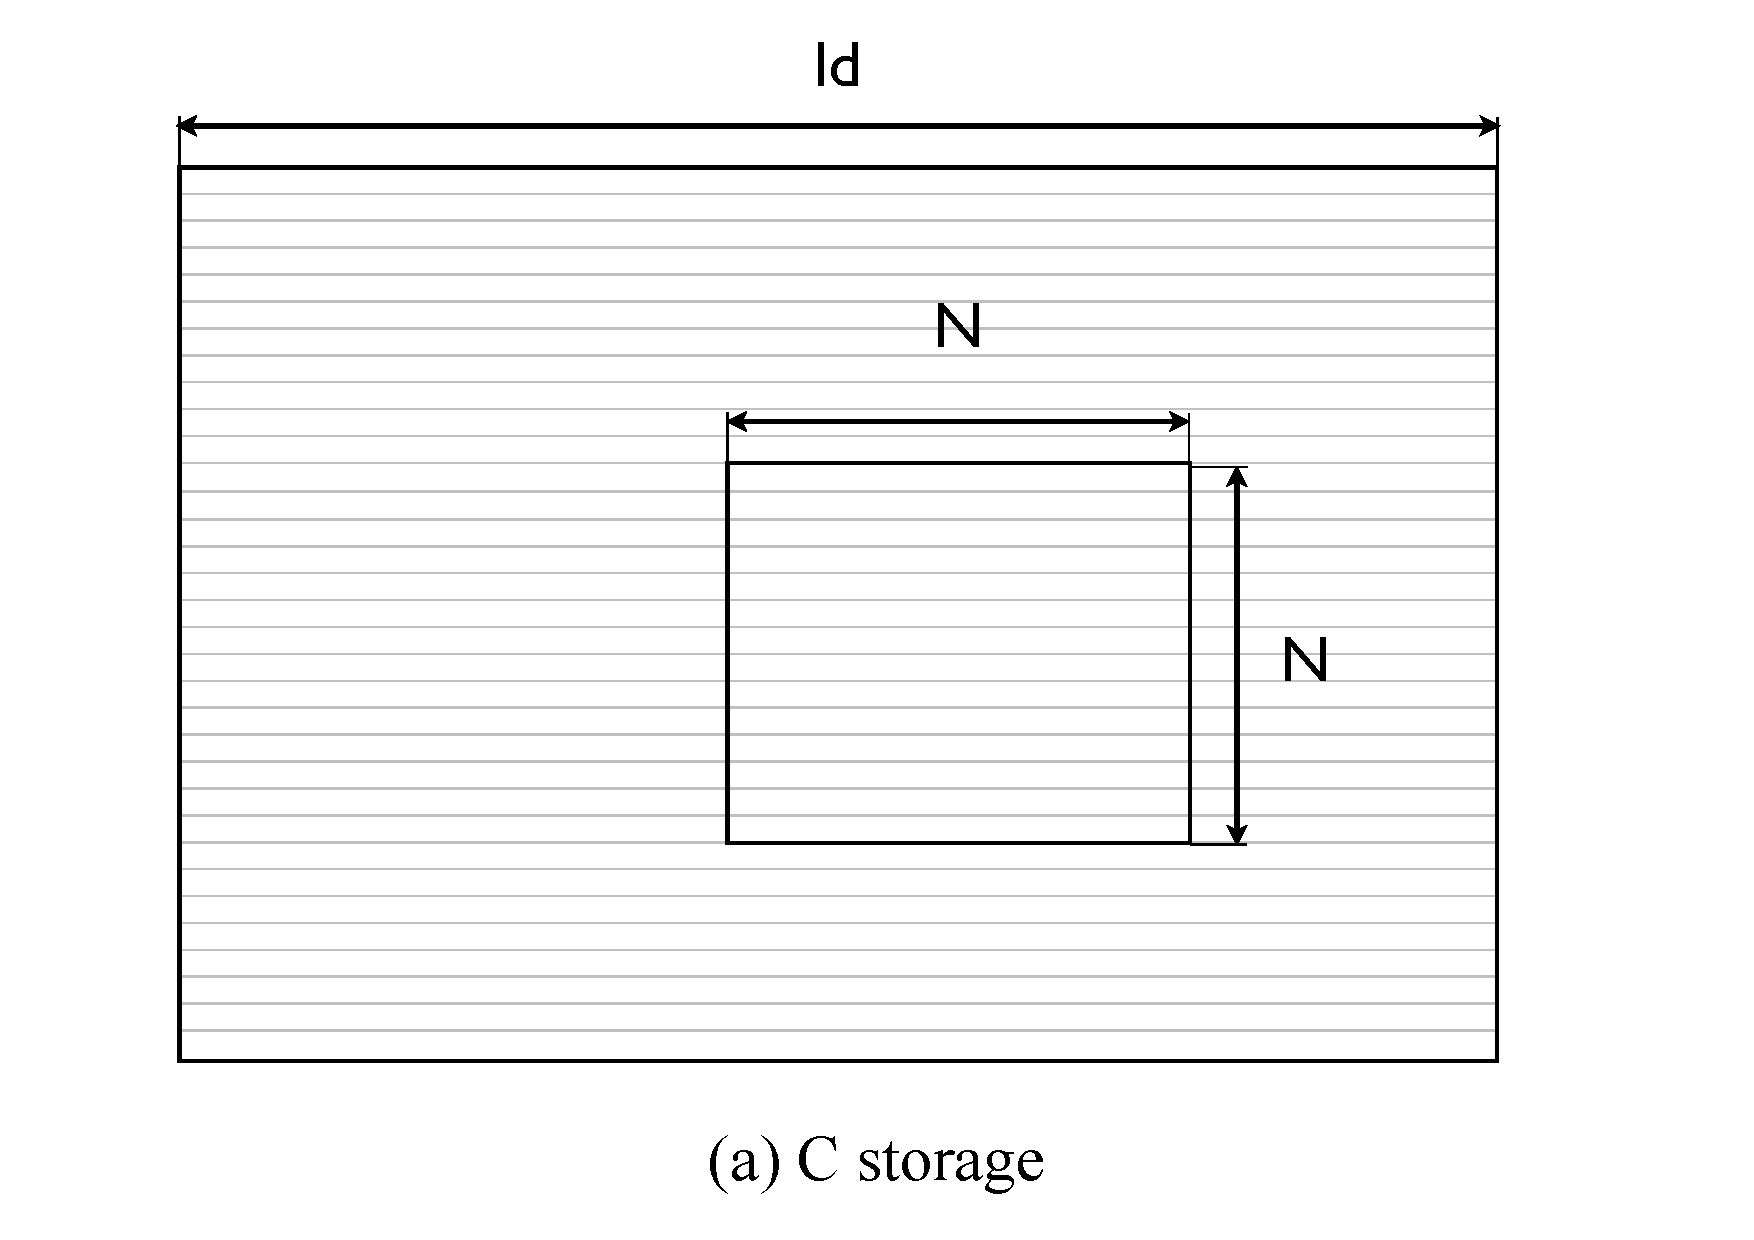
\includegraphics[width=1\linewidth,height=5.8cm]{matrix_C.pdf} 
%\vspace{-0.5cm}
%\noindent{\scriptsize (b) Data flow graph if \textit{cmstep} condition is true.}
\end{center}  
\end{minipage}
\begin{minipage}[t]{0.45\linewidth}
\begin{center}
\vspace{-0.05cm}
\hspace*{0.6ex}
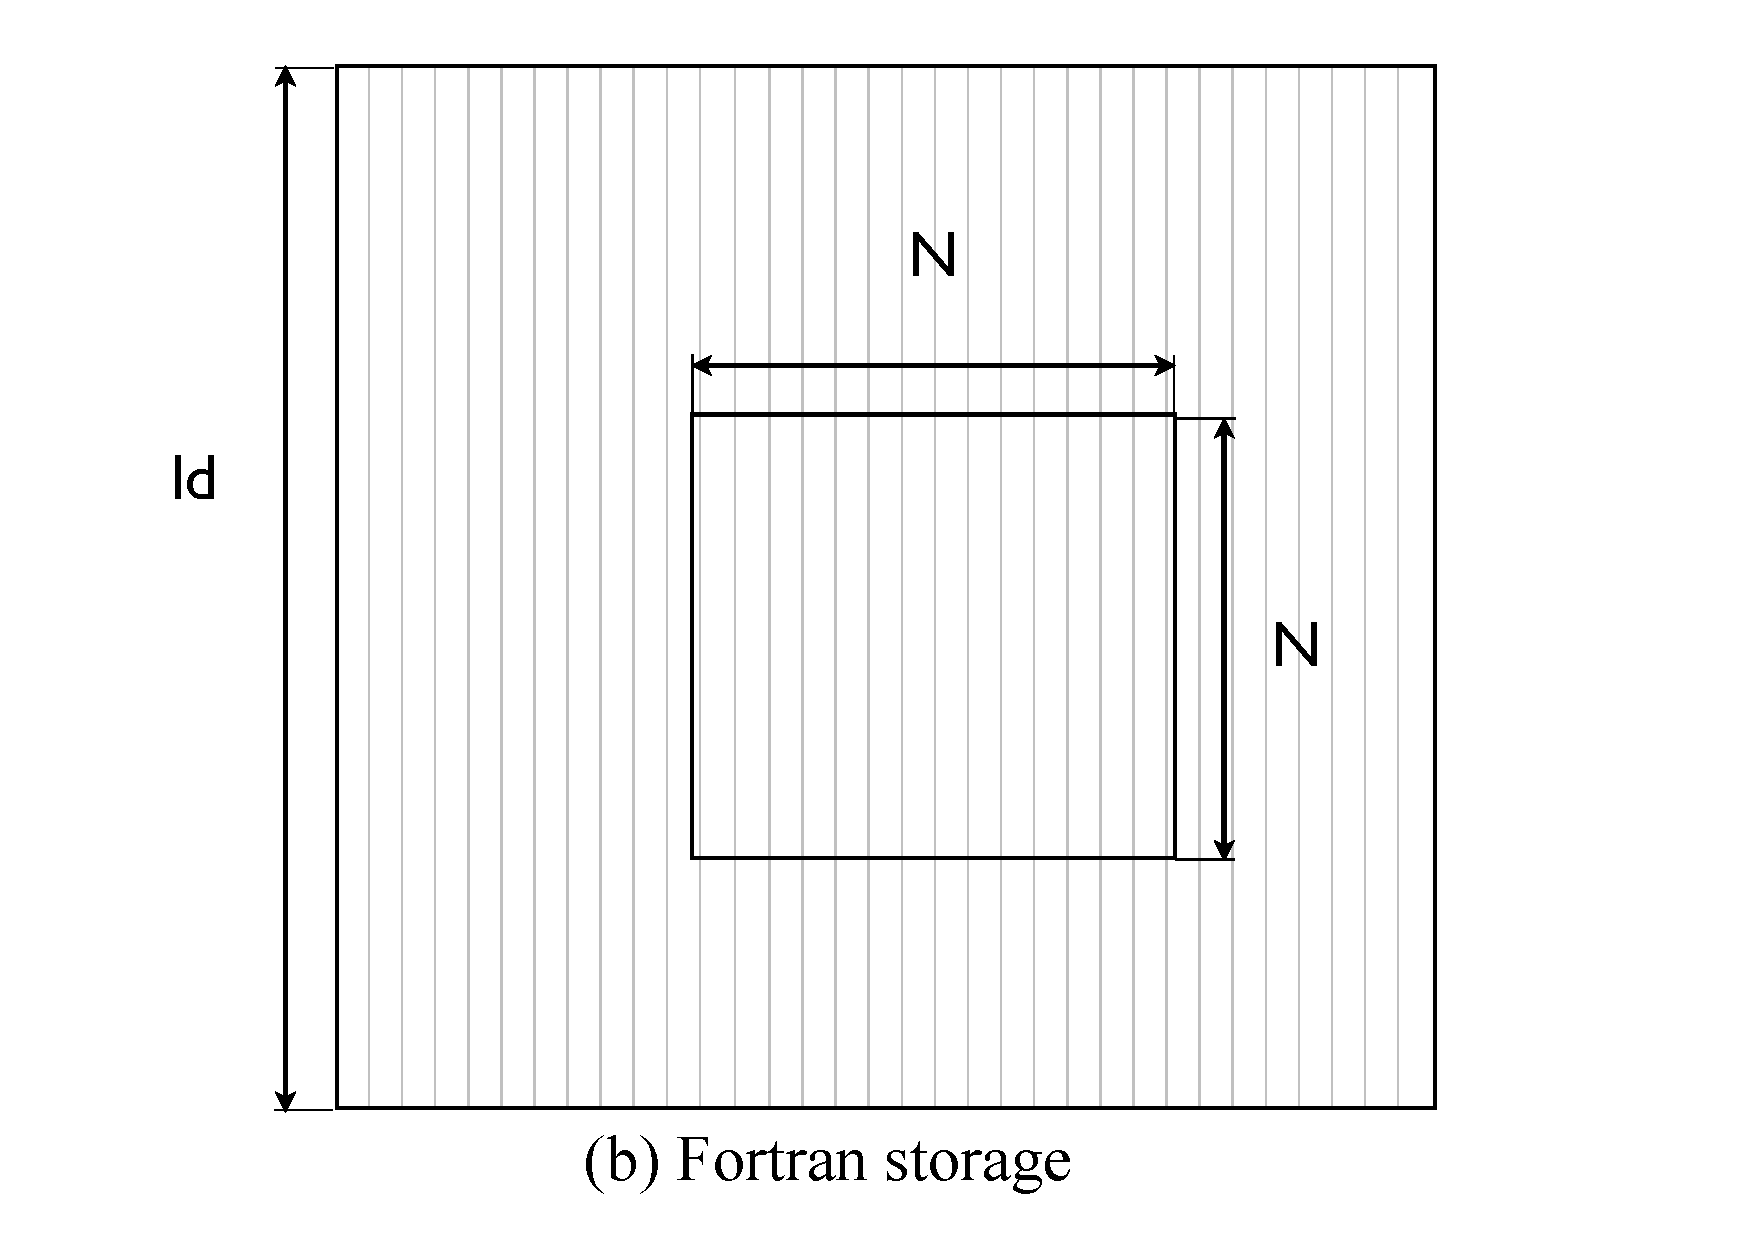
\includegraphics[width=1\linewidth,height=5.8cm]{matrix_F.pdf} 
%\vspace{-0.5cm}
%\noindent{\scriptsize (b) Data flow graph if \textit{cmstep} condition is true.}
\end{center}  
\end{minipage}
\end{center}  
\vspace*{-2ex}
\caption{Two standard storage classes for matrices}
\label{fig:matrix}
\end{figure}

If the leading dimension is not equal to the column dimension (for C storage convention, or row dimension for Fortran convention), it must be specified for 2-dimensional array using the attribute \texttt{ld=<identifier>}. The identifier must be the identifier of a formal parameter.

The storage class (C or Fortran) may be specified in the storage attribute (\texttt{storage=C} in listing of figure~\ref{fig:exmemregion1} at line 5, or \texttt{storage=Fortran}). The default value is the \texttt{C}.

\subsubsection{Passing rule by value}
Any function parameter passed by value must have a value access mode.
In this case, the effective parameter is copied at task's creation time and any modification remains local to the function.

Any C or C++ type may by defined to be passed by value.
The syntax is the following:
\begin{verbatim}
#pragma kaapi task value( <list declaration> )
\end{verbatim}
\texttt{<list declaration>} is a rule in the grammar given in the appendix~\ref{sec:grammar}.

\subsubsection{Passing rule by reference}
Any memory region description in \kaapi must be defined by a C/C++ pointer type formal parameter. At runtime, the pointer, the declaration of the memory region and the access mode (read, write, ...) made by the task allow to detect dependencies.

The syntax of the clause is:
\begin{verbatim}
#pragma kaapi task mode ( <list declaration> )
#pragma kaapi task mode_cw ( operator: <list declaration> )
\end{verbatim}
The access mode name \texttt{mode}�of the clause is given by table~\ref{table:accessmode}.
The previous example accumulate defines 3 arguments. 2 of them are passed by reference: \texttt{array} is an array of size \texttt{n} (known at runtime); \texttt{result} is pointer to one integer.

\paragraph{1-D array.} They are two classical ways to specify a one dimensional array. The first one is by given a base address and a size:
\begin{verbatim}
#pragma kaapi task value(n) read(array[n]) write(result)
void accumulate( int n, int* array, int* result );
\end{verbatim}
The dimension of array must follows the subset of the C grammar for expression. Only reference to variable in the formal parameter list can be done.

The second is to specify a interval between two addresses (as used in the most of the STL algorithms). The syntax use the syntax for interval \texttt{[a:b]}, where \texttt{a} and \texttt{b} are identifiers of formal parameters.
\begin{verbatim}
#pragma kaapi task value(n) read( [begin:end] ) write(result)
void accumulate( int* begin, int* end, int* result );
\end{verbatim}
In the STL, the right bound is not part of the interval and it is called the 'past the last' value of the iterator. The size of the interval is \texttt{b-a}. In C, \texttt{a} and \texttt{b} must be a pointer to any type; in C++ they can also be random access iterators.


\paragraph{2-D array.} 2-D arrays appear de facto in linear algebra subroutines. To allow data structure spliting involved in parallel sub-computations, it is necessary to handle sub sets of 2-D arrays.

\kaapi declaration follows idea of the BLAS storage for dense matrix. 
The syntax of the clause for 2-D array is:
\begin{verbatim}
#pragma kaapi task mode( array[n][m] )
#pragma kaapi task mode( array{ ld=identifier; [n][m] } )
#pragma kaapi task mode( array{ storage=C; \
                                ld=identifier ;  \
                                [n][m] } )
#pragma kaapi task mode( array{ storage=Fortran; \
                                ld=identifier ; \
                                [n][m] } )
\end{verbatim}
Where the \texttt{ld} must be a reference to a formal parameter name. The dimension must follows the sub set of the C grammar for expression. 
C or Fortran keyword are used to specify the storage of the matrix (row major or column major).

All this rules are defined in the grammar of the appendix~\ref{sec:grammar}.


%%%%
\subsubsection{Cumulative access mode}\label{sec:cw}
In \kaapi, it is possible to reduce variable with only associative operator. The commutativity is not required.
A task that required an accumulative semantic with respect to one of its formal parameters, must defined it with the \texttt{reduction} clause in the \texttt{\#pragma kaapi task}. Two tasks having a reduction access mode onto the same memory region are concurrent. 
As depicted in figure~\ref{fig:exaccu},
\begin{figure}[ht]
\hrule\vspace*{1ex}
\begin{center}
\begin{minipage}[t]{0.97\linewidth}
%\scriptsize
\begin{verbatim}
#pragma kaapi task read(array[n]) reduction(+: result) value(n)
void accumulate (int n, int* array, int *result) 
{
   ...
}
\end{verbatim}
\end{minipage}
\end{center}
\vspace*{-1ex}
\hrule
\caption{Kaapi signature for accumulate with reduction}
\label{fig:exaccu}
\end{figure}
The reduction clause specifies the operator to use during concurrent reduction and a list of formal parameters the clause is applied on.
For all the scalar types of the C or C++ language, \kaapi predefines a list of known operators.
For each operator, the neutral element corresponds to the neutral element of the mathematical operator. The list is presented in table~\ref{table:opcumul} follows the same predefined reduction operators in OpenMP-3.0.
\begin{table}[h]
\begin{center}
\small \footnotesize
\begin{tabular}{c|c|c}
               & ~name~ & ~neutral~  \\
\whline
\verb!+! & addition & 0   \\  \hline
\verb!-! & subtraction & 0   \\  \hline
\verb!*! & multiplication & 1    \\  \hline
\verb!&! & bitwise and & \verb+~+0  \\   \hline
\verb!|! & bitwise or & 0  \\   \hline
\verb!^! & bitwise xor & 0  \\   \hline
\verb!&&! & logical and & 1 \\ \hline 
\verb!||! & logical or & 0 \\ \hline 
\end{tabular}
\end{center}
\caption{Predefined cumulative operators.}
\label{table:opcumul}
\end{table}

The user has the possibility to define its own reduction operator using \texttt{\#pragma kaapi declare reduction} clause:
\begin{description}
\item [\texttt{\#pragma kaapi declare reduction}]~\\
\verb!(reduction-identifier : function-name)!\\
\verb![ identity( function-name) ]!\\
The \verb!function-name! must correspond to the name of C/C++ function which must satisfy one of the following signature:
\vspace*{-2ex}\begin{verbatim}
  // For  C++
  void function( typename& result, const typename& value )
  // For C or C++
  void function( typename* result, const typename* value )
\end{verbatim}
\end{description}
The parameter type are inherited from the declaration of the reduction variable in the \texttt{reduction} clause to describe access mode of formal parameter.


In the same way, the identity function is used to initialize a value of a temporary variable to be the neutral of the reduction operator. The identity function signature must be one of the following:
\begin{verbatim}
  // For  C++
  void function( typename& value )
  // For C or C++
  void function( typename* value )
\end{verbatim}

%%%%
\subsubsection{Dependencies between tasks}
Once access modes are defined for the tasks, the runtime is able to detect dependencies between tasks that access to a same memory region.
\begin{description}
\item [Read after Write.] This is also called true dependency. It means that a task is reading a memory region produced by other tasks.
\item [Write after Write.] This is a false dependency. Such dependency is removed using renaming: the two tasks can be executed concurrently if they work on distinct memory region, thus the runtime may allocate distinct memory region.
\item [Write after Read.] This false dependency is also called anti-depedency. Those kinds of dependency are subject to removal in the similar way as write after write dependency.
\end{description}

Note that the \kaapi runtime used a lazy approach to remove false dependencies: if it is necessary to execute concurrently two tasks with false dependencies, then the runtime renames the memory region. Else, the execution is sequential using the task creation order.

In both case, the result of the execution remains the same whatever the execution order between tasks.


%%%%
%%%
\subsection{Directive for synchronization}\label{sec:synchro}

Because task creations that occur at each function call to task function are non blocking instruction, it may be
necessary to synchronize the control flow of the thread that creates tasks with the task executions themselves.

\subsubsection{\#pragma kaapi sync}

The directive forces the synchronization of the current executing control flow with all previously created tasks in the same task's activation frame.

For non recursive task creations, this directive waits until all previously created tasks in the control flow have been completed.

For recursive task creations, the directive waits until all previously created tasks, in the current task activation frame, has been completed.

\subsubsection{\#pragma kaapi sync(<list of views>)}

This directive forces the synchronization of the current executing control flow until the execution of the last created tasks, in the same task activation frame, which writes the memory described by a the list of views.


%%%%
%%%
\subsection{Recursive function call}\label{sec:recursive}

\kaapi allows recursive task creations.
This is illustrated in figure~\ref{fig:recexaccu}, where the accumulate code recursively split the computation until a grain (of 2 here) by creating sub-tasks after splitting the array in two parts. The first created task will accumulate the values \texttt{array[0],...array[n/2-1]} and the second task will accumulate the values \texttt{array[n/2],...,array[n-1]}.
\begin{figure}[ht]
\hrule\vspace*{1ex}
\begin{center}
\begin{minipage}[t]{0.9\linewidth}
%\scriptsize
\begin{verbatim}
#pragma kaapi task read(n, array[n]) reduction(+: result) 
void accumulate (int n, int* array, int *result) 
{
   if (n < 2) *result += array[0] + array[1];
   else {
     accumulate (n/2, array, result);
     accumulate (n-n/2, array+n/2, result);
   }
}
\end{verbatim}
\end{minipage}
\end{center}
\hrule
\caption{Recursive Kaapi accumulate code}
\label{fig:recexaccu}
\end{figure}

This example is simple: no temporary data are required at each level of recursion. This not the case with the academic recursive non optimal computation of the fibonacci number.

\subsubsection{Control of the allocation scope of data}
All data passed by reference to tasks must be valid until the task completion.
For instance, because task creation is a non blocking call the example of figure~\ref{ex:caplante} is incorrect: the automatic variable \texttt{r} will be suppressed before the execution of the task \texttt{g}.
\begin{figure}[ht]
\hrule\vspace*{1ex}
\begin{center}
\begin{minipage}[t]{0.9\linewidth}
%\scriptsize
\begin{verbatim}
1  if (...)
2  {
3    int r; /* store sub result */
4    g(&r, input_values); /* create task*/
5  }
\end{verbatim}
\end{minipage}
\end{center}
\hrule
\caption{Incorrect code}
\label{ex:caplante}
\end{figure}

In that case, the user has two possibilities:
\begin{itemize}
\item Add a synchronization point between line 4 and 5. It enforces the execution waits for the completion of \texttt{g} (left solution in figure~\ref{ex:caplanteplus}).
\item Allocate the data in the same scope as the tasks. In that case, the data is allocated with a scope wide enough to execution of task \texttt{g} (right solution in figure~\ref{ex:caplanteplus}).
\end{itemize}

\begin{figure}[ht]
\hrule\vspace*{1ex}
\begin{center}
\begin{minipage}[t]{0.49\linewidth}
%\scriptsize
\begin{verbatim}
1  if (...)
2  {
3    int r; 
4    g(&r, input_values); 
5    #pragma kaapi sync
6  }
\end{verbatim}
\end{minipage}\vrule~~
\begin{minipage}[t]{0.49\linewidth}
\begin{verbatim}
1  if (...)
2  {
3    #pragma kaapi data alloca(r)
4    int r; 
5    g(&r, input_values); 
6  }
\end{verbatim}
\end{minipage}
\end{center}
\hrule
\caption{Solution for incorrect code of figure~\ref{ex:caplante}}
\label{ex:caplanteplus}
\end{figure}

The syntax of the \texttt{\#pragma kaapi data alloca} is:
\begin{description}
\item [\texttt{\#pragma kaapi data alloca}] \verb!(<list of variables>)!\\
The \verb!<list of variables>! describes a list of automatic variables that hope to be used in task's creations.
\end{description}

The \kaapi name of the directive was chosen with analogy of the \texttt{alloca} function of the C library stdlib.  With sequential C or C++ program, the developper may allocate data in the stack using the \texttt{alloca} function. In that case, the allocation scope is the same as the activation frame where the call to \texttt{alloca} occured.
With \kaapi \texttt{\#pragma kaapi alloca}, the user can allocate data within the same scope as created tasks in the same activation frame.

%%%%
\subsubsection{Example with recursive task's creations}\label{sec:alloca}

%With sequential C or C++ program, the developer may allocate data in the stack using the \texttt{alloca} function. In that case, the scope of allocation is the same as the activation frame where the call to \texttt{alloca} occured.
%With \kaapi, the user may also allocate data within the same scope as created tasks in an activation frame.

To control the allocation scope of automatic variables allocated into the C stack of example in figure~\ref{fig:recaccumalloca}, the programmer has to use the directive \texttt{\#pragma data alloca}  at line 11.
\begin{figure}[ht]
\hrule\vspace*{1ex}
\begin{center}
\begin{minipage}[t]{0.9\linewidth}
%\scriptsize
\begin{verbatim}
1  #pragma kaapi task read(result1, result2) write(result) 
2  void sum (int* result, int * result1, int* result2) 
3  {
4    *result = *result1 + *result2;
5  }

6  #pragma kaapi task read(n, array[n]) write(result) 
7  void accumulate (int n, int* array, int *result) 
8  {
9     if (n < 2) *result += array[0] + array[1];
10    else {
11 #pragma kaapi data alloca(subresult1, subresult2);
12      int subresult1;
13      int subresult2;
14      accumulate (n/2, array, &subresult1);
15      accumulate (n-n/2, array+n/2, &subresult2);
16      sum( result, &subresult1, &subresult2 );
17    }
18 }
\end{verbatim}
\end{minipage}
\end{center}
\hrule
\caption{Accumulate recursive code where the allocation of \texttt{subresult1} and \texttt{subresult2} is 
specify to have the same scope of the spawned task using directive \texttt{\#pragma kaapi alloca}.}
\label{fig:recaccumalloca}
\end{figure}



%\subsection{Definition of complex memory region}
%%
%%The declaration of the list of formal parameters with their access mode is  called the \textbf{task' signature}. The task should also be associated to an entry point called \textbf{task body} which is the function to execution during task execution. A task may have several bodies~\cite{kaapi_europar} depending of the target architecture were to execute it. 
%\textit{TODO. L'impl�mentation ne correspond pas encore � �a: � voir l'int�r�t r��l}
%
%The listing of figure~\ref{fig:recaccumcomplex} presents how to define access mode for the field of a data structure.
%Here the data structure is the struct \texttt{myarray} which defines a size (int) and the data (array of int).
%When the user call the task, it is necessary to define type of each field. Here the fields are passed in \texttt{read} mode.
%\begin{figure}[ht]
%\hrule\vspace*{1ex}
%\begin{center}
%\begin{minipage}[t]{0.9\linewidth}
%%\scriptsize
%\begin{verbatim}
%/* array struct definition */
%typedef struct myarray {
%  int size;
%  int* data;
%} myarray;
%
%#pragma kaapi task value(array.size) read(array.data[array.size]) \
%                   reduction(+: result)
%void accumulate (myarray array, int *result) 
%{
%  int n = array.size;
%  if (n < 2) *result += array.data[0] + array.data[1];
%  else {
%    myarray subarray1 = { n/2, array.data };
%    myarray subarray2 = { n-n/2, array.data + n/2 };
%
%    accumulate ( subarray1, result);
%    accumulate ( subarray2, result);
%  }
%}
%
%int main( int argc, char** argv )
%{
%  /* create and initialize the array */
%  int result;
%  myarray array;
%  array.size = 100;
%  array.data = malloc( 100 * sizeof(int) );
%  for (int i=0; i<100; ++i)
%    array[i] = rand();
%    
%  /* spawn tasks */
%#pragma kaapi parallel
%  {
%    accumulate( array, &result );
%    printresult( &result );
%  }  
%  return 0;
%}
%\end{verbatim}
%\end{minipage}
%\end{center}
%\vspace*{-2ex}
%\caption{Accumulate recursive code with sub shared access mode definitions. The printresult is the task defined in figure~\ref{fig:accummainkaapi}.}
%\hrule
%\label{fig:recaccumcomplex}
%\end{figure}
%
%Note that in this version, because arguments are passed by value, it is not necessary to allocate them in a specific way.
%If the programer wants to pass a pointer to a structure, then the sub arrays used at each recursive call must be defined to be allocated in the same stack as the stack, like in code of figure~\ref{fig:recaccumalloca} by using the \texttt{\#pragma kaapi data alloca} directive.
%
%Because data structure may contains a lot of data field member, it is possible to define the access mode for the whole data structure and refining the access mode for more interesting mode. 
%
%
%

%%%
%%%
\newpage \section{Examples}\label{sec:exp}


\subsection{Fibonacci computation}

\subsubsection{With sync}

\begin{small}
\lstset{numbers=left, numberstyle=\tiny, stepnumber=1, numbersep=5pt}
\lstset{commentstyle=\color{blue}}
\lstset{language=C}
\begin{lstlisting}[frame=tb]
#include <stdio.h>

#pragma kaapi task write(result) value(n)
void fibonacci(long* result, const long n)
{
  if (n<2)
    *result = n;
  else 
  {
    long r1,r2;
    fibonacci( &r1, n-1 );
    fibonacci( &r2, n-2 );
#pragma kaapi sync
    *result = r1 + r2;
  }
}

#pragma kaapi task read(result) 
void print_result( const long* result )
{
  printf("Fibonacci(30)=%li\n", *result);
}

int main()
{
  long result;
#pragma kaapi parallel
  {
    fibonacci(&result, 30);
    print_result(&result);
  }
  return 0;
}
\end{lstlisting}
\end{small}

\subsubsection{Without sync}
\begin{small}
\lstset{numbers=left, numberstyle=\tiny, stepnumber=1, numbersep=5pt}
\lstset{commentstyle=\color{blue}}
\lstset{language=C}
\begin{lstlisting}[frame=tb]
#include <stdio.h>

#pragma kaapi task write(result) read(r1,r2)
void sum( long* result, const long* r1, const long* r2)
{
  *result = *r1 + *r2;
}

#pragma kaapi task write(result) value(n)
void fibonacci(long* result, const long n)
{
  if (n<2)
    *result = n;
  else 
  {
#pragma kaapi data alloca(r1,r2)
    long r1,r2;
    fibonacci( &r1, n-1 );
    fibonacci( &r2, n-2 );
    sum( result, &r1, &r2);
  }
}

#pragma kaapi task read(result) 
void print_result( const long* result )
{
  printf("Fibonacci(30)=%li\n", *result);
}

int main()
{
  long result;
#pragma kaapi parallel
  {
    fibonacci(&result, 30);
    print_result(&result);
  }
  return 0;
}
\end{lstlisting}
\end{small}

\subsubsection{With reduction variable}

\begin{small}
\lstset{numbers=left, numberstyle=\tiny, stepnumber=1, numbersep=5pt}
\lstset{commentstyle=\color{blue}}
\lstset{language=C}
\begin{lstlisting}[frame=tb]
#include <stdio.h>

#pragma kaapi task reduction(+:result) value(n)
void fibonacci(long* result, const long n)
{
  if (n<2)
    *result += n;
  else 
  {
    fibonacci( result, n-1 );
    fibonacci( result, n-2 );
  }
}

#pragma kaapi task read(result) 
void print_result( const long* result )
{
  printf("Fibonacci(30)=%li\n", *result);
}

int main()
{
  long result;
#pragma kaapi parallel
  {
    fibonacci(&result, 30);
    print_result(&result);
  }
  return 0;
}
\end{lstlisting}
\end{small}


\subsection{Cholesky factorization}
This example shows one of the main difference between StartSs programming model is its ability to view sub matrix of matrix without necessity to reallocate the user's data structure.\\

\begin{tiny}
\lstset{numbers=left, numberstyle=\tiny, stepnumber=1, numbersep=5pt}
%%\lstset{commentstyle=\textcolor{blue}}
\lstset{language=C}
\begin{lstlisting}[frame=tb]
#include <cblas.h> 
#include <clapack.h> 


#pragma kaapi task value(Order, Uplo, N, lda) readwrite(A{ld=lda; [N][N]})
int clapack_dpotrf(const enum ATLAS_ORDER Order, const enum ATLAS_UPLO Uplo,
                   const int N, double *A, const int lda);


#pragma kaapi task value(Order, Side, Uplo, TransA, Diag, M, N, alpha, lda, ldb) \
                   read(A{ld=lda; [N][N]}) readwrite(B{ld=ldb; [N][N]})
void cblas_dtrsm(const enum CBLAS_ORDER Order, const enum CBLAS_SIDE Side,
                 const enum CBLAS_UPLO Uplo, const enum CBLAS_TRANSPOSE TransA,
                 const enum CBLAS_DIAG Diag, const int M, const int N,
                 const double alpha, const double *A, const int lda,
                 double *B, const int ldb);

#pragma kaapi task value(Order, Uplo, Trans, N, K, alpha, lda, beta, ldc) \
                   read(A{ld=lda; [N][N]}) \
                   readwrite(C{ld=ldc; [N][N]})
void cblas_dsyrk(const enum CBLAS_ORDER Order, const enum CBLAS_UPLO Uplo,
                 const enum CBLAS_TRANSPOSE Trans, const int N, const int K,
                 const double alpha, const double *A, const int lda,
                 const double beta, double *C, const int ldc);

#pragma kaapi task value(Order, TransA, TransB, M, N, K, alpha, lda, ldb, beta, ldc) \
                   read(A{ld=lda; [M][K]}, B{ld=ldb; [K][N]}) \
                   readwrite(C{ld=ldc; [M][N]})
void cblas_dgemm(const enum CBLAS_ORDER Order, const enum CBLAS_TRANSPOSE TransA,
                 const enum CBLAS_TRANSPOSE TransB, const int M, const int N,
                 const int K, const double alpha, const double *A,
                 const int lda, const double *B, const int ldb,
                 const double beta, double *C, const int ldc);


// Block Cholesky factorization A <- L * L\^t
// Lower triangular matrix, with the diagonal, stores the Cholesky factor.
void Cholesky( double* A, int N, size_t blocsize )
{
  for (size_t k=0; k < N; k += blocsize)
  {
    clapack_dpotrf(
      CblasRowMajor, CblasLower, blocsize, &A[k*N+k], N
    );

    for (size_t m=k+blocsize; m < N; m += blocsize)
    {
      cblas_dtrsm
      (
        CblasRowMajor, CblasLeft, CblasLower, CblasNoTrans, CblasUnit,
        blocsize, blocsize, 1., &A[k*N+k], N, &A[m*N+k], N
      );
    }

    for (size_t m=k+blocsize; m < N; m += blocsize)
    {
      cblas_dsyrk
      (
        CblasRowMajor, CblasLower, CblasNoTrans,
        blocsize, blocsize, -1.0, &A[m*N+k], N, 1.0, &A[m*N+m], N
      );
      for (size_t n=k+blocsize; n < m; n += blocsize)
      {
        cblas_dgemm
        (
          CblasRowMajor, CblasNoTrans, CblasTrans,
          blocsize, blocsize, blocsize, -1.0, 
          &A[m*N+k], N, 
          &A[n*N+k], N, 
          1.0, 
          &A[m*N+n], N
        );
      }
    }
  }
#pragma kaapi sync
}


/* Main of the program
*/
void main( int argc, char** argv )
{
  // matrix dimension
  int N = 32;
  if (argc > 1)
    N = atoi(argv[1]);

  // block count
  int block_count = 2;
  if (argc > 2)
    block_count = atoi(argv[2]);
    
  size_t blocsize = N / block_count;

  double t0, t1;
  double* A = 0;
  if (0 != posix_memalign((void**)&A, 4096, N*N*sizeof(double)))
  {
    printf("Fatal Error. Cannot allocate matrice A, errno: %i\n", errno);
    return;
  }

  // Generate matrix A 
  generate_matrix(A, N);

  // Cholesky factorization of A 
  Cholesky(A, N, blocsize);

  free(A);
  
  return 0;
}
\end{lstlisting}
\end{tiny}

%%%\subsection{Merge Sort}

%%%\subsection{NQueens}

\subsection{2D Histogram}
\begin{tiny}
\lstset{numbers=left, numberstyle=\tiny, stepnumber=1, numbersep=5pt}
%\lstset{commentstyle=\color{blue}}
\lstset{language=C}
\begin{lstlisting}[frame=tb]
#include <stdio.h>
#include <stdlib.h>

/* define the hist level too. assume <= 32. */
#define CONFIG_DATA_LOG2 13
/* dont touch */
#define CONFIG_DATA_DIM (1 << CONFIG_DATA_LOG2)
#define CONFIG_BLOCK_DIM (CONFIG_DATA_DIM / 8)


/* histogram reduction */
#pragma kaapi declare			\
  reduction(hist_redop: reduce_hist)	\
  identity(init_hist)

static void init_hist(unsigned int* p)
{
  *p = 0;
}

__attribute__((unused))
static void reduce_hist(unsigned int* lhs, const unsigned int* rhs)
{
  *lhs += *rhs;
}

#pragma kaapi task			\
  value(bdim, hdim, lda)		\
  read(data{ld = lda; [bdim][bdim]})	\
  reduction(hist_redop: hist[hdim])
static void compute_block_hist
(
 const unsigned int* data,
 unsigned int bdim, /* block dimension */
 unsigned int lda,
 unsigned int* hist,
 unsigned int hdim /* histogram dimension */
)
{
  unsigned int x, y;
  for (y = 0; y < bdim; ++y, data += lda)
    for (x = 0; x < bdim; ++x, ++data)
      ++hist[*data];
}

static void compute_hist
(
 const unsigned int* data,
 unsigned int dim,
 unsigned int* hist
)
{
  static const unsigned int lda = CONFIG_DATA_DIM;
  static const unsigned int block_size =
    CONFIG_BLOCK_DIM * CONFIG_BLOCK_DIM;

  const unsigned int block_count = dim / CONFIG_BLOCK_DIM;
  unsigned int i, j;

  for (i = 0; i < CONFIG_DATA_DIM; ++i)
    init_hist(hist + i);

  for (i = 0; i < block_count; ++i)
  {
    for (j = 0; j < block_count; ++j)
    {
      /* compute start of block */
      const unsigned int* const p =
      	data + i * block_size + j * CONFIG_BLOCK_DIM;
      compute_block_hist
	(p, CONFIG_BLOCK_DIM, lda, hist, CONFIG_DATA_DIM);
    }
  }
}


/* data helpers */
static unsigned int* gen_data(unsigned int dim)
{
  const unsigned int size = dim * dim;
  unsigned int* const data = malloc(size * sizeof(unsigned int));

  /* arrange so that each value appears dim times */
  unsigned int i;
  for (i = 0; i < size; ++i) data[i] = i & (dim - 1);
  return data;
}

static int check_hist(const unsigned int* hist)
{
  unsigned int i;
  for (i = 0; i < CONFIG_DATA_DIM; ++i)
    if (hist[i] != CONFIG_DATA_DIM) return -1;
  return 0;
}


/* main */
int main(int ac, char** av)
{
  static unsigned int hist[CONFIG_DATA_DIM];
  unsigned int* const data = gen_data(CONFIG_DATA_DIM);
  int err;

  if (data == NULL) return -1;

#pragma kaapi parallel
  compute_hist(data, CONFIG_DATA_DIM, hist);

  free(data);

  err = check_hist(hist);
  if (err == -1) printf("invalid\n");

  return err;
}
\end{lstlisting}
\end{tiny}

\subsection{SMPSs examples}

SMPSs is the implementation of the StartSs programming model for multicore architectures.
SMPSs is developed by the Barcelona Supercomputing Center (\url{http://www.bsc.es}) and is freely available for download.

All examples from SMPSs are accepted by the KaCC compiler.
The user may have a look at \url{http://www.bsc.es/plantillaG.php?cat_id=385} to download SMPSs software that contains examples.

\kaapi programming model defines a set of directives which are a superset of the StartSs directives. The appendix~\ref{app:smpss} further details the differences between \kaapi and StartSs/SMPSs.

%%%
%%%
\appendix 

\newpage  \section{C and C++ support}\label{secC++compatibility}


\newpage \section{Grammars}\label{sec:grammar}

In the following grammar, we assume terminal symbols:
\begin{verbatim}
  identifier := [a-zA-Z_][a-zA-Z_0-9]*
  integral := [0-9]+
\end{verbatim}

\subsection{Grammar for description of task's parameters}
The following grammar describes the rules to define access mode for each
parameter in the \verb+#pragma kaapi task+ compiler directive.
\begin{verbatim}
      list_param :=
          access_param
        | access_param list_param
      
      access_param :=
          mode '(' list_declaration ')
       |  mode_cw '(' redop ':' list_declaration ')
      
      list_declaration :=
          range_declaration
        | list_declaration ',' range_declaration
        
      range_declaration :=
          identifier
        | identifier dimension
        | identifier '{' complex_view '}
        | '[' identifier ':' identifier ']'
        | '[' identifier ':' identifier ')'
      
      complex_view :=
          element_view
        | complex_dimension ',' element_view
      
      element_view :=
          'storage' '=' storage_class
        | 'ld' '=' identifier
        | dimension

      mode :=
        | mode_w | mode_r | mode_x | mode_cw
      mode_w :=
          'write'     | 'w'  | 'output'
      mode_r :=
          'read'      | 'r'  | 'input'
      mode_x :=
          'exclusive' | 'x'  | 'inout'
      mode_cw :=
          'reduction' | 'cw'
      mode_v :=
          'value'     | 'v'
      
      redop :=
          '+' | '-' | '*' | '&' | '|' | '^' | '&&' | '||'
        | identifier

      storage_class :=
          'rowmajor'    | 'C' | 'C++'
        | 'columnmajor' | 'Fortran'      
\end{verbatim}
\subsubsection{Note on access mode}
Most of the different access modes (\verb+mode_xx :=+ rules) have three formats: long, short and a format compatible with the  SMPSs programming model. 
If the reduction operator for an \verb+reduction+ access mode is left unspecified, they the default operator is \verb'+' for all the scalar type (integral value and floating point value). 
For other instance of type or class that does not have the \verb'+' operator defined, then this is an compiler error. The default identity operator is: for scalar value (integral value and floating value) to set the value '0' which is the neutral element with respect to the associative default \verb'+' operator. For other type or class which have a defined \verb'+' operator, then the neutral is assumed to be set by calling the default constructor.

\subsubsection{Note on range declaration}

In the range declaration rule, the programmer has to opportunity to define the set of memory address that the task will access. 
The set of memory address may have any shape. This set serves to detect dependencies between tasks. The implementation has currently 2 limits:
\begin{enumerate}
\item The grammar limits the shape to continuous D dimensional arrays, 
with an implementation limit to 2D data structures (see next section about the grammar).
\item The detection of dependency between tasks uses a special memory address of the range declaration which is named the \textbf{referent}. This address is the address of the identifier in case of the D-dimensional format. And for 1D definition using the format \verb+[identifier .. identifier]+ this is the memory address given by the value of the first identifier (a pointer).
\end{enumerate}

The grammar may be extended in the future in order to take into account more complex shape declaration.


\subsubsection{Dimension definition}\label{ref:dimensiongrammar}
The dimension in range specification is described by the following grammar. Expression rules in the grammar is a subset of the C expression rules.
\begin{verbatim}
      dimension :=
          one_dimension 
        | one_dimension dimension

      one_dimension :=
          '[' expression ']'

      expression :=
        additive_expression

      additive_expression :=
          multiplicative_expression
        | additive_expression '+' multiplicative_expression
        | additive_expression '-' multiplicative_expression
        
      multiplicative_expression
          cast_expression
        | multiplicative_expression '*' cast_expression
        | multiplicative_expression '/' cast_expression
        | multiplicative_expression '%' cast_expression

      cast_expression
          unary_expression
        | '(' type_name ')' cast_expression

      unary_expression
          primary_expression
        | SIZEOF unary_expression
        | SIZEOF '(' type_name ')'
      
      primary_expression
          identifier
        | integral
        | '(' expression ')'
\end{verbatim}


\subsection{Grammar for reduction operator}
The compiler directive \verb+#pragma kaapi declares <reduction_declaration>+ follows the next grammar. This grammar may be extended to match the OpenMP directive to declare reduction operators using pseudo variable.
\begin{verbatim}
      reduction_declaration :=
          reduction_definition
        | reduction_definition identity_definition
        
       reduction_definition :=
        | 'reduction' '(' identifier ':'  function_name ')'

       identity_definition :=
          'identity'  '(' function_name  ')'
        | 'identity'  '(' '{' initializer-list '}' ')'
\end{verbatim}
The role of the identity declaration is to specify the initialization a variable with the value that corresponds to the neutral element with respect to the reduction operator. For instance: \texttt{0} for operator \texttt{+} over scalar type.
For user's defined type, this function should be defined. In C++, if the identity function is not defined, the C++ empty constructor is used to initialize this value. In C, the default identity function set to zero the data structure. 

The signature of the reduction function must be:
\begin{verbatim}
// For C or C++
void function_name( type_name* result, const type_name* value ); 

// For C++
void function_name( type_name& result, const type_name& value ); 
\end{verbatim}
The signature for the identity function follows the same rule:
\begin{verbatim}
// For C or C++
void identity_name( type_name* value ); 

// For C++
void identity_name( type_name& value ); 
\end{verbatim}


\subsection{Grammar for \texttt{data alloca} directive}
The following grammar is involved in the directive
\begin{verbatim}
#pragma kaapi data alloca <list of variables>
\end{verbatim}
\begin{verbatim}
      list_of_variables :=
          identifier
        | list_of_variables ',' identifier 
\end{verbatim}
This directive must be defined in a basic block before the definition of automatic variable.
This is a compiler error to pass a non automatic name (\textit{e.g.} global variable) or to declare the pragma after the definition of the variable.


%%%
%%%
\newpage
\section{KaCC compiler and runtime options}\label{sec:compilo}

\subsection{Compilation process with KaCC}

The compilation process with KaCC of a file is the following:
\begin{enumerate}
\item Each \kaapi directive  that begins \texttt{\#pragma kaapi} is interpreted and the code is rewritten to call function of the \kaapi library. Invalid use of \kaapi directive and some warning are outputed.
\item The backend compiler (C or C++) is called on the rewritten code to generate an object file.
\item To create an executable, KaCC passes the \kaapi library to the linker.
\end{enumerate}


\subsection{KaCC options}
The KaCC compiler recognizes all the options of Gcc compiler suite (gcc, g++) and add an extra option:
\begin{description}
\item [-\,-keep]: keep the intermediate files. For each file, 2 intermediate files are generated. The first one is prefixed by \texttt{kaapi-} and is the translation of the file with replacement of function call by task creation.
\end{description}


\subsection{Backend compiler selection}
The backend compiler is the default C or C++ compiler defined during the installation step (see options with \texttt{configure --help}). It can be changed at configuration by setting the environment variables \texttt{CC} and \texttt{CXX}.

\subsection{Runtime environment variables}
\begin{description}
\item [KAAPI\_CPUSET]: if defined, and if the operating system support it, then the variable specifies the set of core to use in \kaapi program. If no defined, the operating system decides to schedule \kaapi threads onto the cores.
The syntax is a list of core identifiers or a range of core identifiers:
\begin{verbatim}
KAAPI_CPUSET=1,2,6,8,21
KAAPI_CPUSET=0:11,20:31
\end{verbatim}
The identifier corresponds to system identifier for the core.
\item [KAAPI\_CPUCOUNT]: if defined, the variable specifies the number of cores to use. This number should be less than the number of cores specified with \texttt{KAAPI\_CPUSET}.
\end{description}


%%%
%%%
\newpage
\section{ SMPSs task model compatibility}\label{app:smpss}

A parallel  SMPSs program running on a multicore is composed of several threads sharing the process address space. The threads execute tasks which may shared values in the address space, that we call thread shared memory.
A task is a function call: a function and the list of its effective parameters. 
In  SMPSs~\cite{smpss-manual} the definition of a task is based on the annotation of the C function definition. Figure~\ref{fig:accumulatesmpss} illustrates the methodology: the original sequential code \verb+accumulate+ is annotated to be a task if compiled with  SMPSs (\verb+#pragma css task+). Each formal parameter is described by the access the task performs: \verb+input+ means that the task requires it to be ready before execution; \verb+output+ means that the task will produce it. And \verb+inout+ for the both. A depicted  in the code, a formal parameter may be defined with a size in order to identify the memory region accessed by the task.
\begin{figure}[ht]
\begin{center}
\hrule\vspace*{1ex}
\begin{minipage}[t]{0.9\linewidth}
%\scriptsize
\begin{verbatim}
#pragma css task input(n, array[n]) output(result) 
void accumulate (int n, int* array, int *result) 
{
  int sum = 0; 
  for (int i=0; i<n; ++i)
    sum = sum + array[i];
  *result = sum;
}
\end{verbatim}
\end{minipage}
\end{center}
\hrule
\vspace*{-1ex}
\caption{ SMPSs Accumulate code}
\label{fig:accumulatesmpss}
\end{figure}

All tasks are created asynchronously: the callee returns immediately after the task creation, before its execution. SMPSs only guarantees that true data flow dependencies (read after write) are verified: SMPSs ensures that a task consuming a value produced by an other task will be executed in order. Two tasks without direct or indirect data flow dependencies can be executed out of order. To ensure serialization, SMPSs defines two kinds of barrier: a global barrier that waits until all previously created tasks have been executed; a local barrier that waits until a list of values has been produced.

The SMPSs programming model must be initialized before (\texttt{\#pragma css init} / \texttt{\#pragama css finish}), and allows reduction with locking mechanisms~\cite{smpss-manual}.


\subsection{Compatibility}

The \kaapi compiler is allowed to parse and execute correctly all the SMPSs directives without any change in the source code. Moreover, due to its extended syntax to define memory region, \kaapi can be used where SMPSs requires source code modification (for instance in all  inplace SMPSs factorization algorithms -LU, Cholesky, QR, ...-).

The semantic of reduction variable in \kaapi allows to avoid locking mechanism at the expense of a memory copy.



\newpage \bibliographystyle{splncs03}
\bibliography{rt-kaapi.bib}

\end{document}

\endinput
%%
%% End of file `squelette-rr.tex'.
